\documentclass{article}
\usepackage[utf8]{inputenc}
\usepackage{txfonts} % https://www.ctan.org/tex-archive/fonts/txfonts
\usepackage{pgf, tikz}
\usepackage[margin=0.5in]{geometry}
\usetikzlibrary{arrows, automata}

\title{Causality exercises 1: http://bayes.cs.ucla.edu/BOOK-2K/slides-hw1.pdf}
\author{Lucas Wiman}
\date{August 2020}
\setlength{\parindent}{0pt}
\newcommand{\given}{\ |\ }
\newcommand{\hr}{\centerline{\rule{19cm}{0.4pt}}}
\begin{document}

\maketitle

\hr

\textbf{Exercise 1:} Prove that the graphoid properties are satisfied if we interpret $\left(X\Perp Y | Z \right)$ to mean ``all paths from a subset $X$ of nodes are intercepted by a subset $Z$ of nodes''. The graphoid properties are:

\textit{\textbf{Symmetry:}} $(X \Perp Y \given Z) \Rightarrow (Y \Perp X \given Z)$.

\textit{\textbf{Decomposition:}} $(X \Perp YW \given Z) \Rightarrow (X \Perp Y \given Z)$.

\textit{\textbf{Weak union:}} $(X \Perp YW \given Z) \Rightarrow (X \Perp Y \given ZW)$.

\textit{\textbf{Contraction:}} $(X \Perp Y \given Z)\ \&\ (X \Perp W \given ZY) \Rightarrow (X \Perp YW \given Z)$.

\textit{\textbf{Intersection:}} $(X \Perp W \given ZY)\ \&\ (X \Perp Y \given ZW) \Rightarrow (X \Perp YW \given Z)$.

\hr
\bigskip

\textbf{Interpretation}:
\begin{itemize}
    \item Here a ``path'' means an undirected path in a directed graph. If we interpret it to mean a directed path, then symmetry would fail on the following graph:

    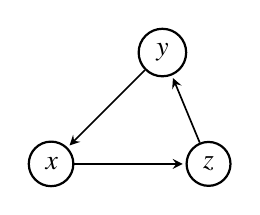
\begin{tikzpicture}[
            > = stealth, % arrow head style
            shorten > = 1pt, % don't touch arrow head to node
            auto,
            node distance = 2cm, % distance between nodes
            semithick % line style
        ]

        \tikzstyle{every state}=[
            draw = black,
            thick,
            fill = white,
            minimum size = 4mm
        ]

        \node[state] (x) {$x$};
        \node[state] (y) [above right of=x] {$y$};
        \node[state] (z) [right of=x] {$z$};

        \path[->] (x) edge node {} (z);
        \path[->] (z) edge node {} (y);
        \path[->] (y) edge node {} (x);

    \end{tikzpicture}

    Then for \textit{directed} paths and $X=\{x\}$, $Y=\{y\}$ and $Z=\{z\}$, we have that every path from $X$ to $Y$, it must be intercepted by an element of $Z$ (i.e. $\left(X\Perp Y \given Z\right)$, but there is a path from $Y$ to $X$ which does not intercept $Z$.
\item For a path to ``intercept" must mean something other than ``shares a node with", since otherwise ``intersection" would fail. Consider the following graph:

    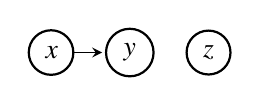
\begin{tikzpicture}[
            > = stealth, % arrow head style
            shorten > = 1pt, % don't touch arrow head to node
            auto,
            node distance = 1cm, % distance between nodes
            semithick % line style
        ]

        \tikzstyle{every state}=[
            draw = black,
            thick,
            fill = white,
            minimum size = 4mm
        ]

        \node[state] (x) {$x$};
        \node[state] (y) [right of=x] {$y$};
        \node[state] (z) [right of=y] {$z$};

        \path[->] (x) edge node {} (y);
    \end{tikzpicture}
    
    Now let $X=\{x\}$, $Y=W=\{y\}$ and $Z=\{z\}$. Then with the ``has a node in common" definition of "intercepted", the left hand side of the ``Intersection" axiom is satisfied, but the right hand side is not. There is a unique path from $X$ to $Y$ that always includes the vertex $y\in Y=W$, and that path intercepts $ZY$ (since in intercepts $Y$) and $ZW$, since it intercepts $W$.
    
    A reasonable definition that seems consistent with the rest of the text is that a set of nodes $Z$ \textit{intercepts} a path $P$, if there is a $z\in Z$ in the path, but it is not an endpoint.
\end{itemize}
\textbf{Proof:} 

\textit{\textbf{Symmetry:}} Assume that $(X \Perp Y \given Z)$, and let $P$ be a path from $Y$ to $X$. Since the path is undirected, reversing $P$ yields a path $P'$ from $X$ to $Y$.  Since $(X \Perp Y \given Z)$, $P'$ must be intercepted by $Z$. Therefore $P$ is intercepted by $Z$. Since $P$ was arbitrary, we have $(Y \Perp X \given Z)$, as desired.

\textit{\textbf{Decomposition:}} Assume $(X \Perp YW \given Z)$. Since every path from $X$ to $Y$ is also a path from $X$ to $YW\supseteq Y$, it must be intercepted by $Z$, as desired.

\textit{\textbf{Weak union:}} Assume $(X \Perp YW \given Z)$. Let $P$ be any path from X to Y. Then $P$ is also a path from $X$ to $YW\subseteq Y$, and therefore must be intercepted by $Z$. Since $Z\subseteq ZW$, $P$ is also intercepted by $ZW$. So since $P$ was arbitrary, we have $(X \Perp Y \given ZW)$, as desired.

\textit{\textbf{Contraction:}} Assume $(X \Perp Y \given Z)$ and ($X \Perp W \given ZY)$.  Let $P$ be a path from $X$ to $YW$, and let $n\in YW$ be the terminal node. Then $n\in Y$ or $n\in W$. If the former, then $Z$ must intercept $P$ since we assumed $(X \Perp Y \given Z)$. If $n\in W$, then since $X \Perp W \given ZY)$, $P$ is intercepted by $Z$ or by $Y$. If $Z$, then we are done. If $Y$, then $n_i\in P$ is an element of $Y$ for some $i$. This subpath of $P$ is then a path from $X$ to $Y$, which must be intercepted by $Z$ by assumption. That means that $P$ is also intercepted by $Z$. In either case, $P$ is intercepted by $Z$, so we have: $(X \Perp YW \given Z)$.

\textit{\textbf{Intersection:}} Assume (1) $(X \Perp W \given ZY)$ and (2) $(X \Perp Y \given ZW)$, but that $(X \not \Perp YW \given Z)$. Then there is a path $P$ from $X$ to $YW$ which is not intercepted by $Z$. Let $P_0$ denote the \textit{shortest} such path. If $P$ terminates in $W$, then by (1) it is intercepted by $ZY$. $P$ is not intercepted by $Z$, so it must be intercepted by $Y$ at some point in the interior of the path, say at node $i < |P|$. But then $n_0,n_1,\ldots,n_i$ is also a path from $X$ to $YW$ that is strictly shorter than $P$, contradicting that $P$ is the shortest path for which independence fails. The case where $P$ terminates in $Y$ is similar, and follows by symmetry.

\end{document}
